\section{Aufbau und Durchf"uhrung}
	\label{sec:durchfuehrung}

	\subsection{Vermessung elastisch gebogener St"abe} % (fold)
	\label{sub:beschreibung_einer_apparatur_zur_vermessung_elastische_gebogener_st_abe}
	
		\begin{figure}[!h]
			\centering
			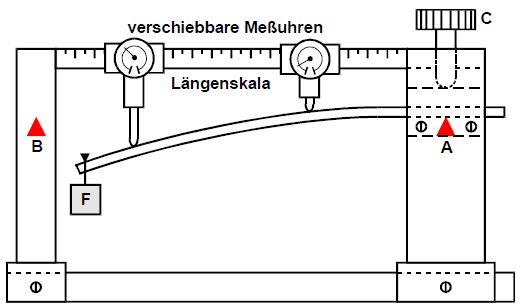
\includegraphics[width = 13cm]{img/messung1.JPG}
			\caption{Schematische Darstellung einer Apparatur zur Vermessung elastisch gebogener St"abe. \cite{anleitung}}
			\label{fg:messung1}
		\end{figure}

		Zur Bestimmung des Elastizit"atsmoduls durch eine Biegungsmessung wird ein Versuchsaufbau nach Abb. \ref{fg:messung1} verwendet. Es ist bei diesem Aufbau m"oglich den Stab entwede einseitig auf dem Fu"spunkt A oder beidseitig auf den Fu"spunkten A und B zu befestigen. Es ist nun m"oglich, je nach Messung, ein Gewicht entweder am Stabende oder in der Stabmitte zu befestigen.

		Zur Messung der Durchbiegung $D(x)$ werden zwei Messuhren benutzt. Diese bestehen aus einem federnden Tastenstift und sind so in der Lage Verschiebungen eines Objektes zu messen. Diese sind auf der X-Achse verschiebbar, sodass eine Messung an verschiedenen Stellen $x$ m"oglich ist.

		Es wirkt auch eine Kraft $F$ auf den Stab ohne das ein Gewicht angeh"angt wurde. Diese Durchbiegung $D_\mathrm{0}(x)$ muss von den Durchbiegungen der anschlie"senden Messungen als Offset abgezogen werden.

		Das Gewicht soll so gew"ahlt werden, dass die maximale Durchbiegung zwischen 3 und 7 mm liegt.

	\subsection{Messung der Schallgeschwindigkeit in St"aben} % (fold)
	\label{sub:messung_der_schallgeschwindigkeit_in_st_aben}
	
		\begin{figure}[!h]
			\centering
			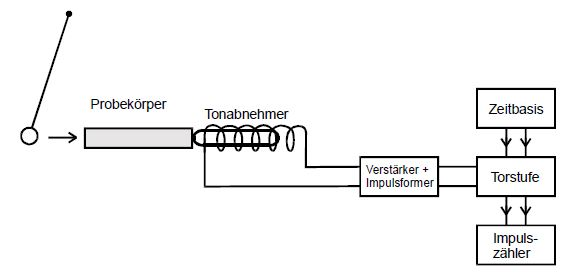
\includegraphics[width = 13cm]{img/messung2.JPG}
			\caption{Schematische Darstellung einer Apparatur zur Messung der Laufzeit eines Schallimpulses in einem stabf"ormigen Probenk"orper. \cite{anleitung}}
			\label{fg:messung2}
		\end{figure}

		Zur Bestimmung der Schallgeschwindigkeit in St"aben wird ein Versuchsaufbau nach Abb. \ref{fg:messung2} verwendet.
		Die elastische Deformation wird durch einen Aufprall mit einer Stahlkugel auf einer Stirnseite der Kugel erzeugt. Der Schallimpuls l"auft durch den Stab hindurch und trifft auf die andere Stirnfl"ache. Dort wird der Schallimpuls in einen elektrischen Impuls umgewandelt. Dieser wird Verst"arkt und eine elektronische Torstufe ge"offnet, sodass die Impulse an einen Impulsz"ahler weitergeletiet werden. Der gr"o"sere Teil der Schallwelle wird jedoch reflektiert und trifft nach kurzer Zeit ein zweites Mal auf das Ende des Stabes. Dieser schlie"st die Torstufe und der Impulsz"ahler zeigt die doppelte Laufzeit des Schallimpulses an. Durch das bet"atigen eines Schalters kann so auch die doppelte Laufzeit eines zehnfach reflektierten Impulses gemessen werden.

		Der Probestab muss anschlie"send gewogen und ausgemessen werden.

	\subsection{Messprogramm} % (fold)
	\label{sub:messprogramm}
	
		Zun"achst wird die Durchbiegung $D(x)$ in Abh"angigkeit von der Distanz $x$ vom Einspannungsort f"ur je einen zylindrischen und rechteckigen Querschnitt bei einseitiger Einspannung gemessen.

		Anschlie"send wird die Messung bei beidseitiger Einspannung wiederholt.

		Weiterhin wird die Laufzeit des Schallimpulses in den zuvor ausgemessenen Probest"abe bestimmt.

		Abschlie"send werden die Probest"abe und die Belastungsgewichte ausgemessen und gewogen.